\chapter{Validação, conclusões e trabalhos futuros}

Para assegurar-se da relevância das categorias de lições aprendidas mapeadas no capítulo anterior, elas foram validadas por profissionais com experiência em adoção ágil atuantes do mercado de TI brasileiro. Além disso, neste capítulo encontra-se o fechamento da pesquisa, com suas conclusões e possíveis trabalhos futuros.

\section{Método de validação}

Após uma revisão de literatura baseada no método de revisão sistemática sobre artigos publicados em revistas e conferências científicas, complementada por  uma pesquisa exploratória de relatos de experiência nas principais conferências nacionais e internacionais no assunto, um conjunto de lições aprendidas foram coletadas. As mesmas foram agrupadas considerando suas similaridades, em 14 categorias/aspectos específicos.

Com o intuito de validar a relevância dessas lições aprendidas propostas por esta pesquisa, um questionário foi elaborado para coletar a opinião de profissionais que vivenciaram a adoção organizacional da abordagem ágil. São 15 questões de múltipla escolha cujo foco é a criticidade de cada categoria/aspecto para que a adoção de Ágil em empresas de desenvolvimento de software ocorra com sucesso.

\subsection{Perfil dos profissionais consultados}

Para ter um melhor controle com relação à competência e ao nível de experiência dos profissionais consultados, o questionário não foi disponibilizado publicamente. Foram recebidas 20 respostas de profissionais que têm em média 14 anos de experiência com desenvolvimento de software e cerca de 8 anos com Ágil. A Tabela \ref{tab:mini-cvs} mostra um pouco sobre aqueles que se identificaram (isto não foi obrigatoriamente solicitado no formulário).

\begin{tabularx}{\linewidth}{ | p{4cm} | X | } \hline \textbf{Nome} & \textbf{Resumo} \\ \hline
	Luca Bastos & Engenheiro, empreendedor por 17 anos e desenvolvedor desde os tempos dos cartões perfurados. Organizador e palestrante no Agile Brazil 2012 e 2013. Keynoter no TWBRAway Day 2012. Palestras: CaipiraAgile 2012, TDC 2012, Qcon 2011, AgileBrazil 2011, TDC 2011, RubyConf 2010, Qcon 2010, TDC 2010 e outros. Atualmente trabalha na ThoughtWorks \\ \hline
	Celso Martins & Atuando no mercado de TI desde 1994, tive os primeiros contatos com o desenvolvimento ainda em 1985, com 7 anos de idade. Tendo passado por grandes empresas, como Embratel, Accenture, Oi, XP Investimentos, hoje atuo como consultor da Crafters Software Studio, ajudando a GVT no processo de transição para gestão ágil. Também tenho me dedicado, de forma teórica e prática, ao assunto mudança organizacional nos últimos 2 anos. Especialista em Lean, Kanban, Scrum, Management 3.0, Sistemas Complexos, ToC, disponho de uma caixa de ferramentas interessante para ajudar as empresas a realizar a mudança para a gestão moderna de uma forma suave e com o menor impacto possível. Nas horas vagas, sou organizador de eventos voltados à Ágil, como o Agile Trends \\ \hline
	Felipe Furtado & Possui mestrado em Ciências da Computação pelo Centro de Informática da UFPE na área de métricas e produtividade. Atualmente é doutorando no CIn em metodologias ágeis e modelos de maturidade, gerente de projetos do C.E.S.A.R, coordenador da pós-graduação em gestão ágil de projetos do C.E.S.A.R.edu e docente do mestrado profissional em engenharia de software. Com 16 anos na área de desenvolvimento de software, foi coordenador da garantia da qualidade de software e do SEPG (Software Engineering Process Group) onde adquiriu experiência na área de engenharia de software com ênfase em qualidade de software e gestão de projetos \\ \hline
	Paulo Caroli & Agilista e protagonista da ThoughtWorks Brasil, Paulo Caroli possui mais de quinze anos de experiência em desenvolvimento de software, com passagem em várias corporações no Brasil, Índia e EUA. Em 2000, conheceu o Extreme Programming e, desde então, tem focado sua experiência em processos e práticas de Gestão e Desenvolvimento Ágil. Ingressou na ThoughtWorks em 2006 e ocupou os cargos de Agile Coach, Trainer, e Gerente de Projetos. Possui os títulos de Bacharel em Ciência da Computação e M.S. em Engenharia de Software, ambos da PUC-Rio \\ \hline
	Marcos Garrido & Quase duas décadas de experiência em projetos de tecnologia e atuando como Product Owner em projetos ágeis desde 2008. Além disso, é professor da disciplina de Métodos Ágeis do MBA em Gestão de Projetos da PUC-RIO. Garrido é um membro ativo das comunidades Ágil e Lean, com forte interesse pelos desafios que envolvem a gestão de produtos. Participou como palestrante em um grande número de eventos nacionais e internacionais, com destaque para os Scrum Gatherings de São Paulo, Munich e Orlando, além do Agile Brazil, Ágiles e Agile Rio. Nos últimos anos, tem se envolvido profundamente com o movimento Lean Startup. Garrido é Mestre em Administração com ênfase em Marketing pela PUC-RIO e possui as certificações CSPO, CSM, CSD e CSP pela Scrum Alliance, além de ser Facilitador certificado de Management 3.0 \\ \hline
	Célio Santana & Doutor em Engenharia de Software pela Universidade Federal de Pernambuco (UFPE). Professor na UFPE e consultor em melhoria de processos \\ \hline
	Dairton Bassi & Possui mestrado em Engenharia de Software e bacharelado em Ciência da Computação pelo IME-USP. Co-fundador da Agile Alliance Brazil, Co-criador do Agile Brazil e Coordenador Geral do Agile Brazil 2012. Envolvido com agilidade há 10 anos, foi CTO da Dafiti e, como consultor, implantou metodologias ágeis em inúmeras empresas \\ \hline
	João Paulo Novais & Engenheiro de Software com mais de 10 anos de experiência. Analista de Negócio no SERPRO, Agile Coach e organizador de eventos da Comunidade Ágil como Agile Brazil e Agile Trends \\ \hline
	Renato Willi & Tem trabalhando com desenvolvimento de software a cerca de 12 anos, sendo os últimos 9 coordenando times através de metodologias ágeis. Atualmente é associado da SEA Tecnologia, uma empresa com mais de 10 anos de estrada. Renato também trabalha como organizador e/ou palestrante em vários eventos nacionais sobre metodologias ágeis (Agile Brazil, Maré de Agilidade, QCon, TDC, etc.), além de escrever artigos para blogs e revistas do ramo e colaborar com projetos voluntários de tradução de livros técnicos\\ \hline
	\captionsetup{justification=centering}
	\caption{Resumo sobre alguns profissionais da área de TI que responderam o formulário e se identificaram}
	\label{tab:mini-cvs}
\end{tabularx}

\subsection{Questionário: perguntas e respostas}

\subsubsection{Qual nível de prioridade você daria para a experiência, treinamento e aprendizado dos envolvidos?}

\begin{figure}[H]
	\centering
	\captionsetup{justification=centering}
	\makebox[\textwidth]{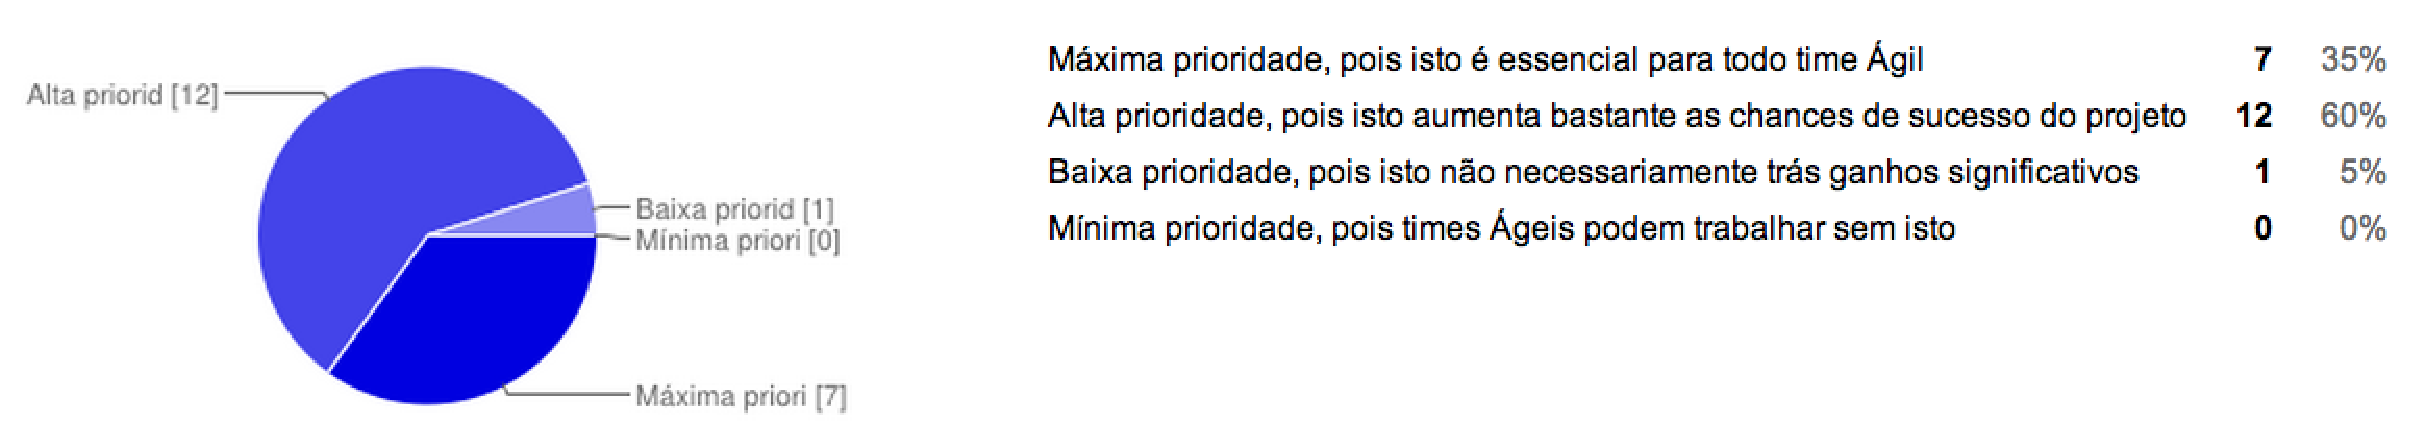
\includegraphics[width=\textwidth]{capitulos/validacao/figuras/exp.eps}}
	\caption{Contabilização das respostas referentes à criticidade da categoria de LAs ``Experiência, treinamento e aprendizado"}
	\label{fig:result-exp}
\end{figure}

\nomenclature{LAs}{Lições aprendidas} %

\subsubsection{Qual nível de prioridade você daria para o planejamento e gerenciamento do backlog do projeto?}

\begin{figure}[H]
	\centering
	\captionsetup{justification=centering}
	\makebox[\textwidth]{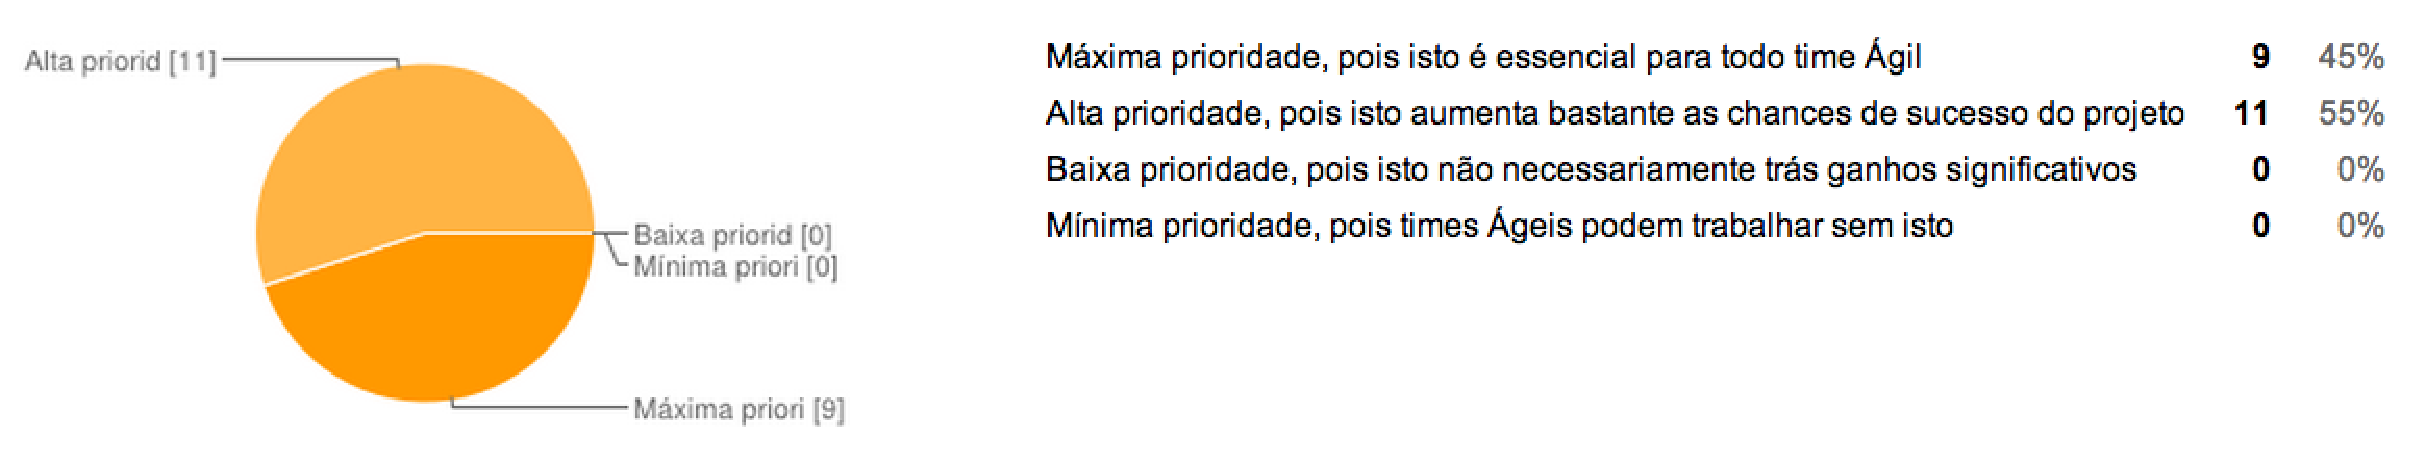
\includegraphics[width=\textwidth]{capitulos/validacao/figuras/backlog.eps}}
	\caption{Contabilização das respostas referentes à criticidade da categoria de LAs ``Planejamento e gerenciamento de backlog"}
	\label{fig:result-backlog}
\end{figure}

\subsubsection{Qual nível de prioridade você daria para o apoio gerencial e dos clientes?}

\begin{figure}[H]
	\centering
	\captionsetup{justification=centering}
	\makebox[\textwidth]{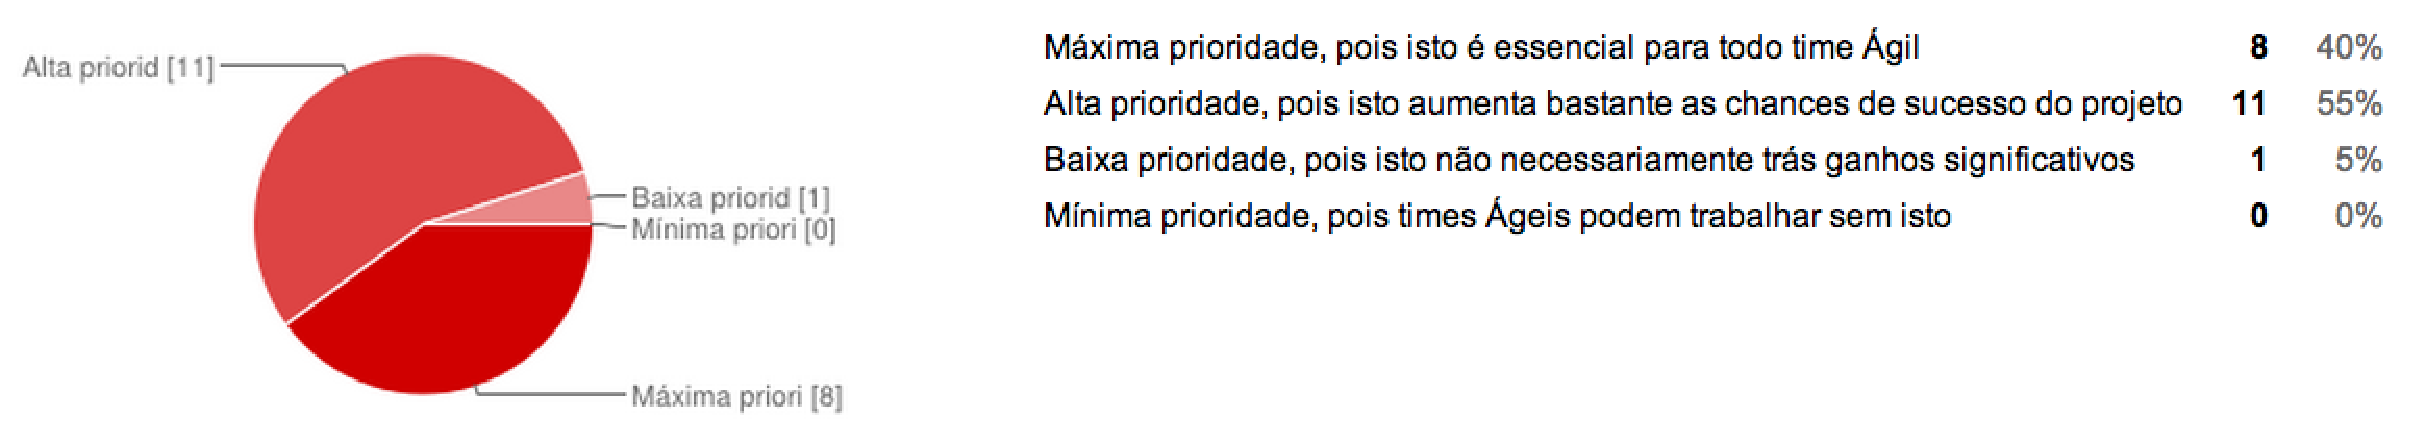
\includegraphics[width=\textwidth]{capitulos/validacao/figuras/apoio.eps}}
	\caption{Contabilização das respostas referentes à criticidade da categoria de LAs ``Apoio gerencial e dos clientes"}
	\label{fig:result-apoio}
\end{figure}

\subsubsection{Qual nível de prioridade você daria para a capacidade de customização e adaptabilidade do projeto?}

\begin{figure}[H]
	\centering
	\captionsetup{justification=centering}
	\makebox[\textwidth]{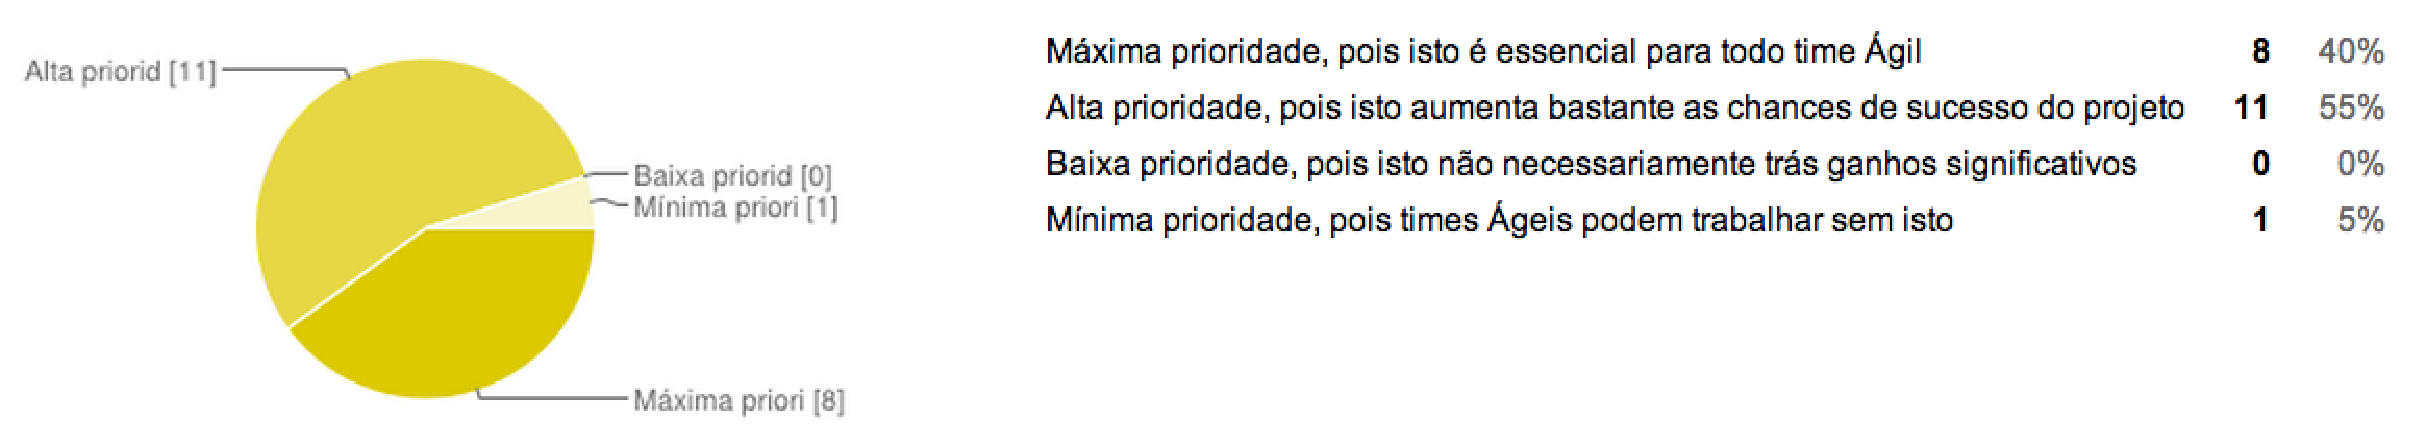
\includegraphics[width=\textwidth]{capitulos/validacao/figuras/adaptabilidade.eps}}
	\caption{Contabilização das respostas referentes à criticidade da categoria de LAs ``Customização e adaptabilidade"}
	\label{fig:result-adaptabilidade}
\end{figure}

\subsubsection{Qual nível de prioridade você daria para o nível de confiança do time?}

\begin{figure}[H]
	\centering
	\captionsetup{justification=centering}
	\makebox[\textwidth]{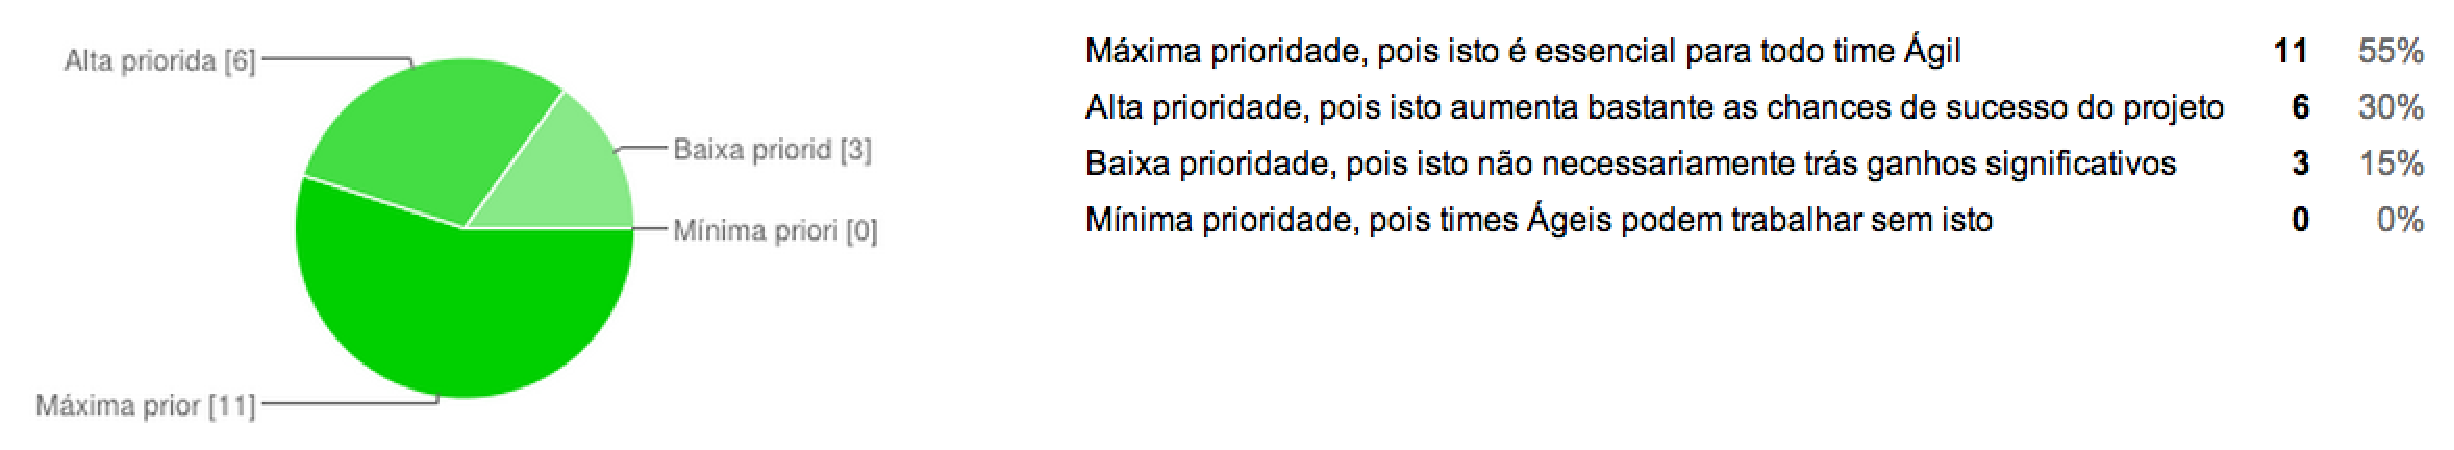
\includegraphics[width=\textwidth]{capitulos/validacao/figuras/confianca.eps}}
	\caption{Contabilização das respostas referentes à criticidade da categoria de LAs ``Confiança do time"}
	\label{fig:result-confianca}
\end{figure}

\subsubsection{Qual nível de prioridade você daria para o nível de engajamento, comprometimento, disciplina e trabalho em equipe dos integrantes do projeto?}

\begin{figure}[H]
	\centering
	\captionsetup{justification=centering}
	\makebox[\textwidth]{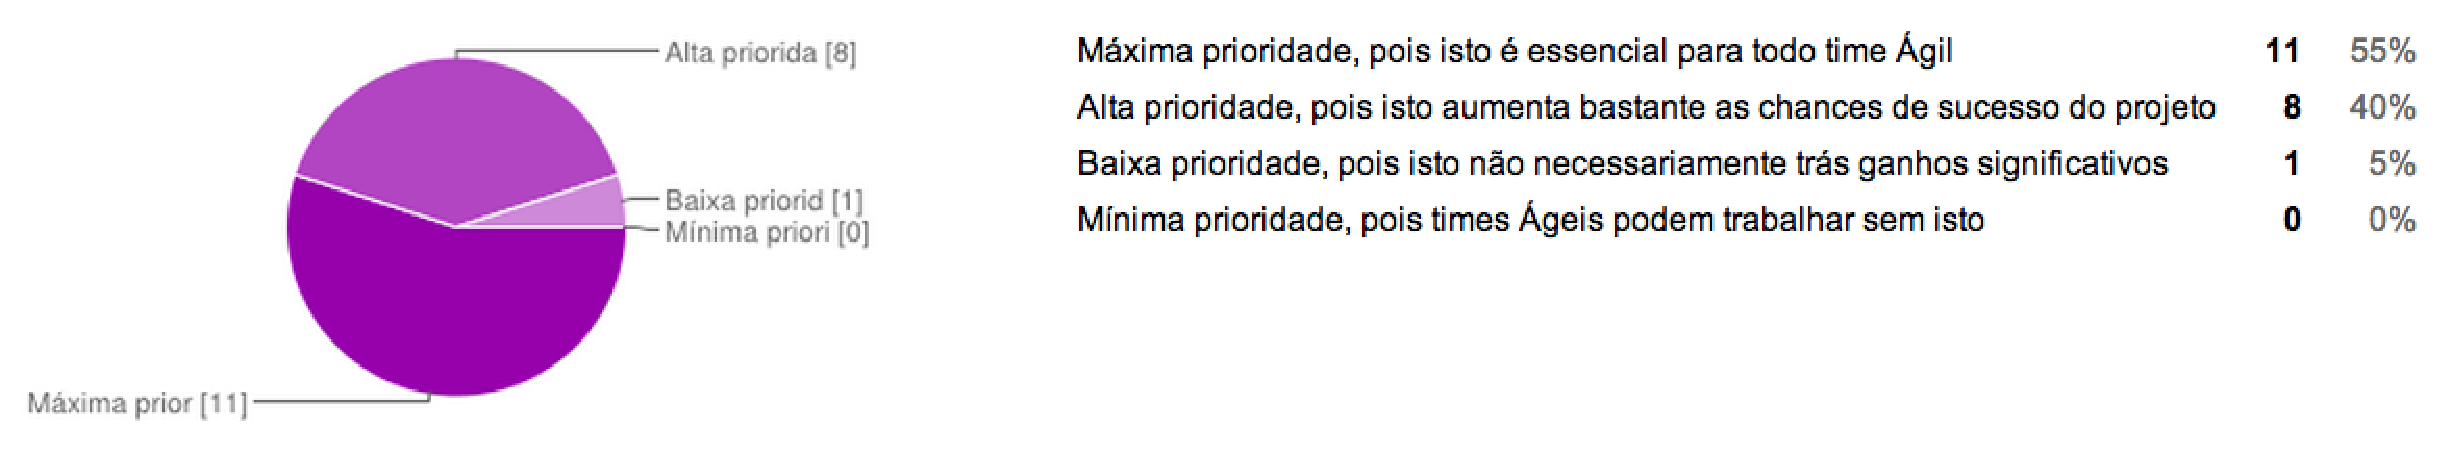
\includegraphics[width=\textwidth]{capitulos/validacao/figuras/engajamento.eps}}
	\caption{Contabilização das respostas referentes à criticidade da categoria de LAs ``Engajamento, comprometimento, disciplina e trabalho em equipe"}
	\label{fig:result-engajamento}
\end{figure}

\subsubsection{Qual nível de prioridade você daria para os aspectos técnicos e tecnológicos utilizados?}

\begin{figure}[H]
	\centering
	\captionsetup{justification=centering}
	\makebox[\textwidth]{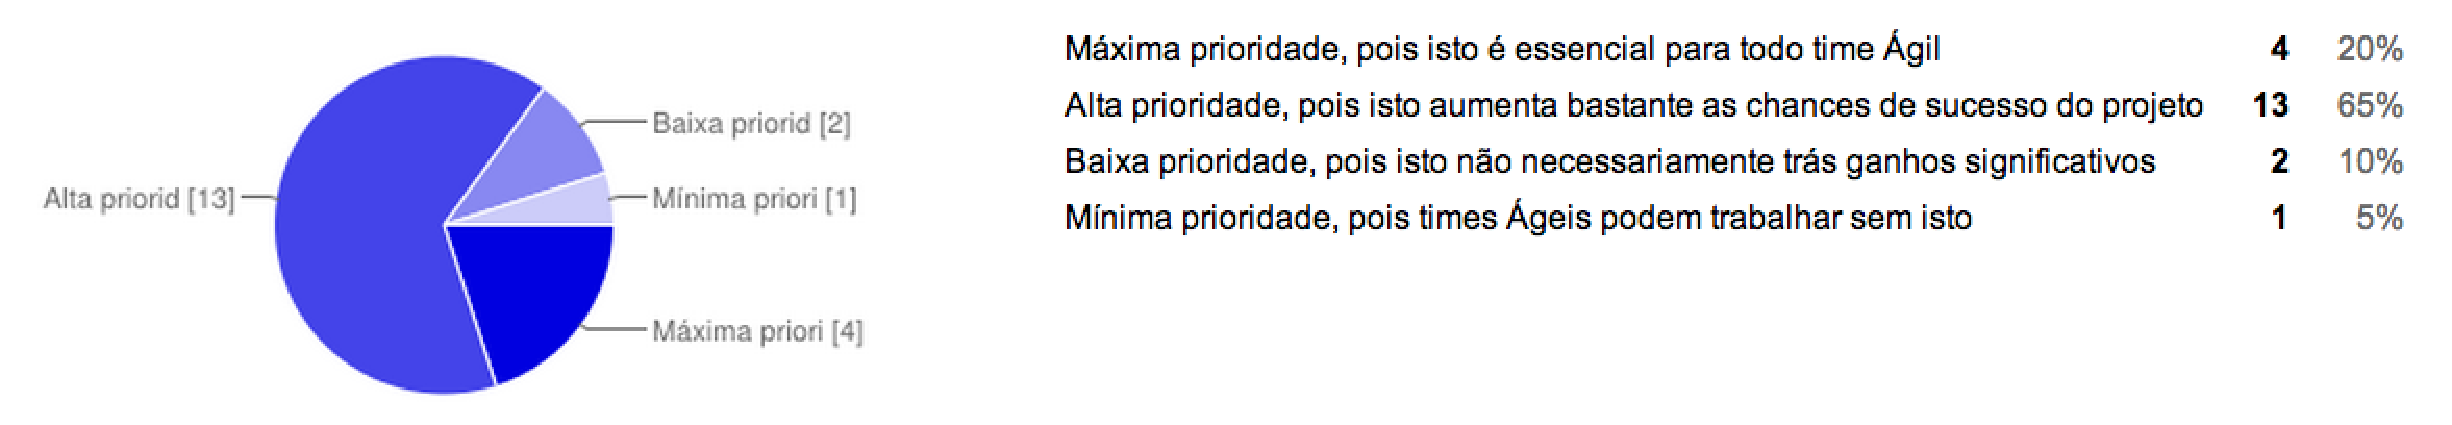
\includegraphics[width=\textwidth]{capitulos/validacao/figuras/tech.eps}}
	\caption{Contabilização das respostas referentes à criticidade da categoria de LAs ``Aspectos técnicos e tecnológicos"}
	\label{fig:result-tech}
\end{figure}

\subsubsection{Qual nível de prioridade você daria para o hábito do compartilhamento de conhecimento dentro e fora do projeto?}

\begin{figure}[H]
	\centering
	\captionsetup{justification=centering}
	\makebox[\textwidth]{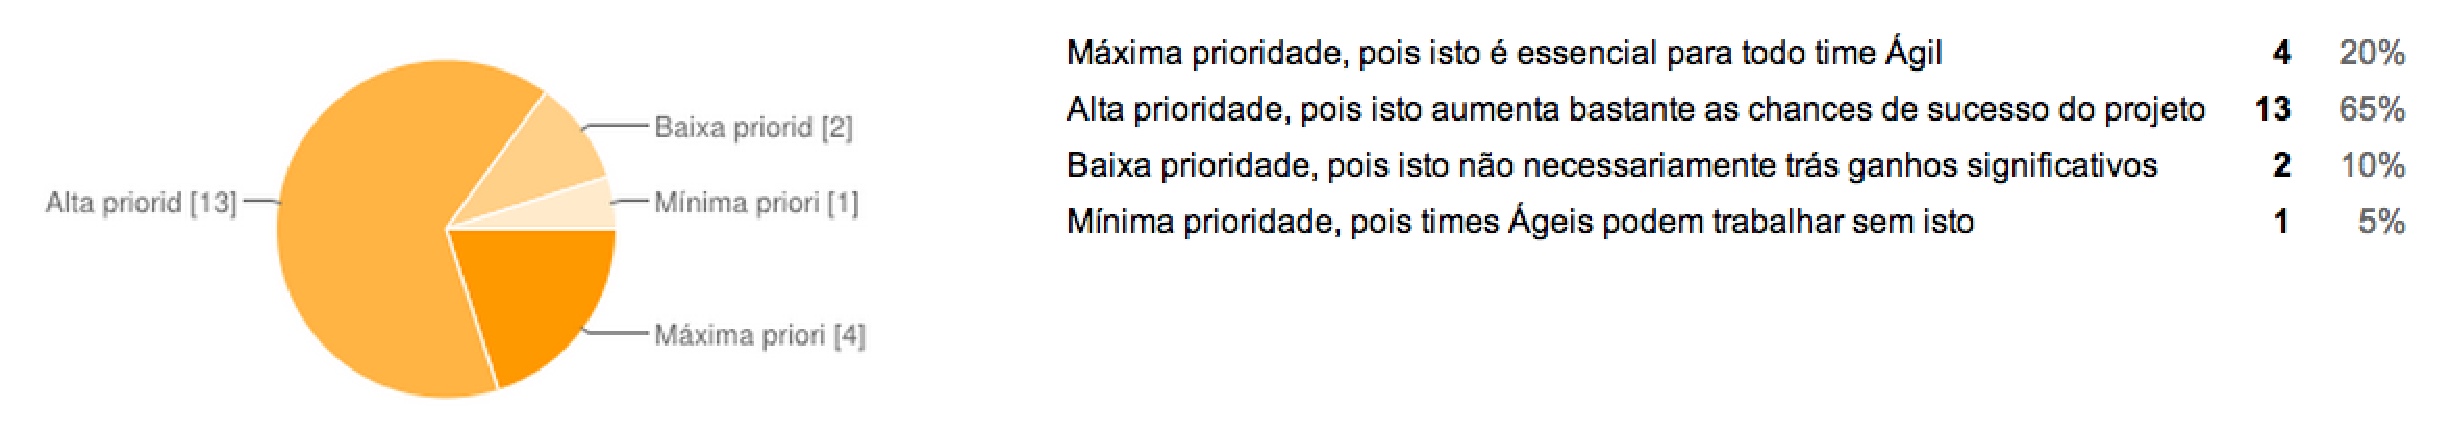
\includegraphics[width=\textwidth]{capitulos/validacao/figuras/conhecimento.eps}}
	\caption{Contabilização das respostas referentes à criticidade da categoria de LAs ``Compartilhamento de conhecimento"}
	\label{fig:result-conhecimento}
\end{figure}

\subsubsection{Qual nível de prioridade você daria para a velocidade de entrega e a produtividade da equipe?}

\begin{figure}[H]
	\centering
	\captionsetup{justification=centering}
	\makebox[\textwidth]{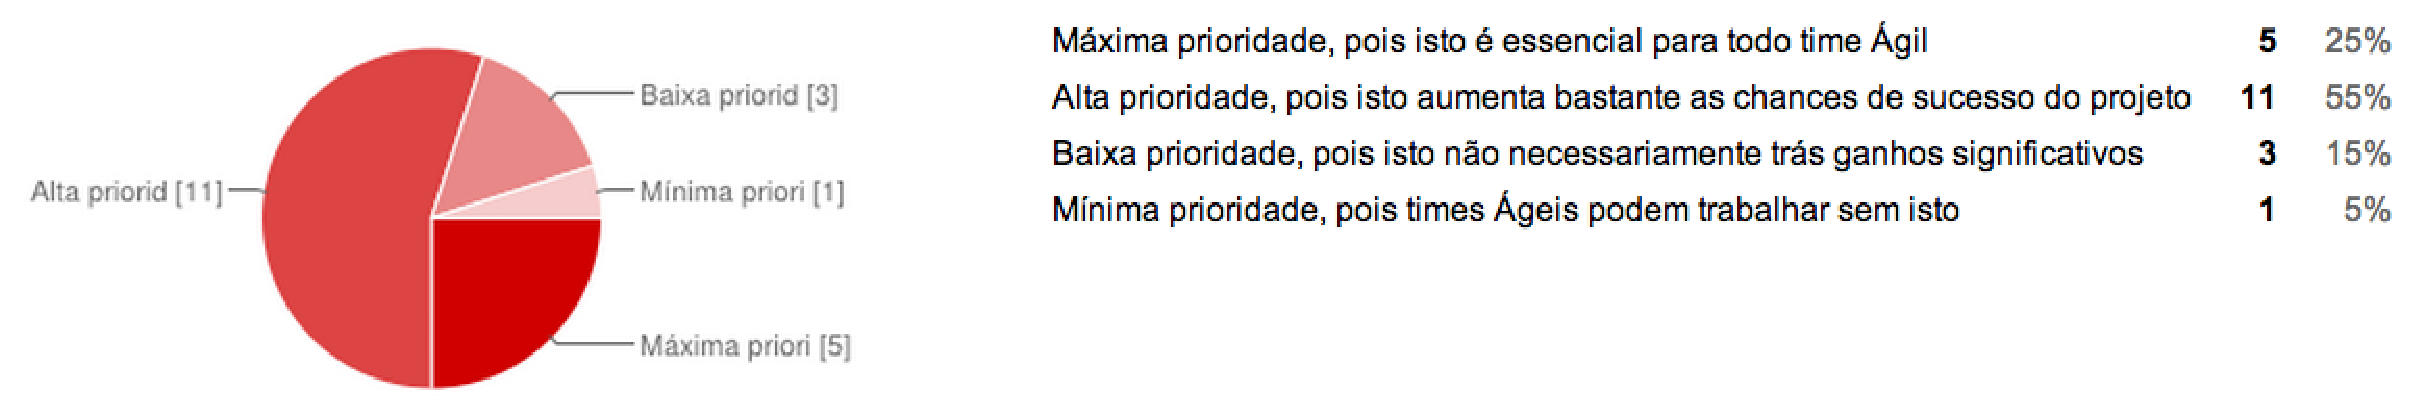
\includegraphics[width=\textwidth]{capitulos/validacao/figuras/produtividade.eps}}
	\caption{Contabilização das respostas referentes à criticidade da categoria de LAs ``Velocidade de entrega e produtividade"}
	\label{fig:result-produtividade}
\end{figure}

\subsubsection{Qual nível de prioridade você daria para a busca pela melhoria na qualidade do produto final?}

[Graph goes here]

\subsubsection{Qual nível de prioridade você daria para os esforços com a quebra de paradigma necessária para a implementação de Ágil?}

[Graph goes here]

\subsubsection{Qual nível de prioridade você daria para o esforço para se lidar com comunicação remota?}

[Graph goes here]

\subsubsection{Qual nível de prioridade você daria para o alinhamento dos Princípios Ágeis com a cultura da organização?}

[Graph goes here]

\subsubsection{Se você tivesse que selecionar apenas 5 das categorias relacionadas anteriormente, quais você ressaltaria como as mais críticas para serem consideradas por uma organização na adoção da abordagem ágil?}

[Graph goes here]

\section{Conclusões}


\section{Trabalhos futuros}
